\chapter{Results} \label{ch:results}

The first intuitive analysis is a correlation to identifying possible predictors of residency. As we want to model the behavior of the traffic, and we assume that the behavior of the residents should be different from the tourists' behavior, we correlate the residence label against all the other variables. We assign a label of 1 if the vehicle is registered in Pampaneira, Capileira or Bubión (registered resident) and 0 otherwise. Our results reveal several variables that showed non-significant correlations (correlation less than 0.2): avg\_visit\_POQ, std\_visit\_POQ, and population, which have been removed (see in \cref{fig:resident_corr}). \cref{tab:outliers} shows the mean and standard deviation for a selection of uncorrelated variables between two groups: registered residents and non-registered individuals. The variable visit\_POQ, which relates to the time of each visit to the area, has a high standard deviation (std\_visit\_POQ) for registered residents, which could indicate the existence of residents who go out more often and others less often. Furthermore, the mean values (avg\_visit\_POQ) of this variable (visit\_POQ) do not differ much between the two groups. As for the population size variable, there are other villages with a similar size to that of the three villages under study. Hence, the three removed variables are less relevant than the rest in predicting whether a vehicle is a resident of the study area or not.

\begin{figure}
\begin{center}
	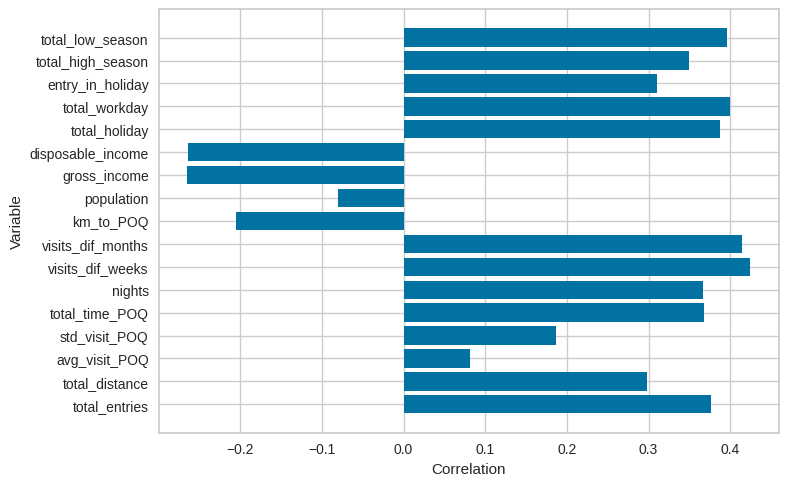
\includegraphics[width = 0.9 \linewidth]{Images/resident_corr.png}
\end{center}
	\caption{\label{fig:resident_corr} Correlation between the registered resident label and the rest of the variables.}
\end{figure}

\begin{table}[]
\centering
\resizebox{\columnwidth}{!}{%
\begin{tabular}{ccccccccc}
\hline
\textbf{}            & \multicolumn{2}{c}{nights}         & \multicolumn{2}{c}{total\_distance} & \multicolumn{2}{c}{total\_entries}     & \multicolumn{2}{c}{entry\_in\_holiday}  \\ \hline
                     & Residents         & Others         & Residents          & Others         & Residents           & Others           & Residents          & Others             \\ \hline
mean                 & 158.47            & 19.99          & 205.82             & 13.60          & 19.46               & 2.35             & 4.26               & 0.72               \\
std                  & 72.37             & 48.07          & 238.52             & 47.78          & 23.57               & 6.58             & 5.49               & 1.70               \\ \hline
\multicolumn{1}{l}{} & \multicolumn{2}{c}{gross\_income}  & \multicolumn{2}{c}{km\_to\_POQ}     & \multicolumn{2}{c}{visits\_dif\_weeks} & \multicolumn{2}{c}{total\_high\_season} \\ \hline
                     & Residents         & Others         & Residents          & Others         & Residents           & Others           & Residents          & Others             \\ \hline
mean                 & 16,084            & 25,007.07      & 1.02               & 374.73         & 4.57                & 1.48             & 27.53              & 3.84               \\
std                  & 0.00              & 7671.19        & 0.59               & 486.97         & 4.03                & 1.97             & 14.75              & 9.00               \\ \hline
\multicolumn{1}{l}{} & \multicolumn{2}{c}{total\_holiday} & \multicolumn{2}{c}{avg\_visit\_POQ} & \multicolumn{2}{c}{std\_visit\_POQ}    & \multicolumn{2}{c}{population}          \\ \hline
                     & Residents         & Others         & Residents          & Others         & Residents           & Others           & Residents          & Others             \\ \hline
mean                 & 52.54             & 6.83           & 23.60              & 10.54          & 20.26               & 4.15             & 406.66             & 19,8175.90         \\
std                  & 23.71             & 15.06          & 34.85              & 31.87          & 23.35               & 16.05            & 121.16             & 56,7183.30    \\ \hline   
\end{tabular}%
}
\caption{Mean and std. deviation for registered residents and rest of individuals in dataset.}
\label{tab:outliers}
\end{table}

\subsection*{Preprocessing and Dimension reduction results: Normalization selection}


Although the preprocessing and dimension reduction stages are performed sequentially, they are interdependent, so we will describe them together. 

PCA technique handles the linear correlations of the original variables to create the principal components. However, we observed that the prior removal of highly correlated variables improves the variance explained by PCA and the scatter plots displaying the PCA component. Hence, we plot in \cref{fig:matrix} the correlation matrix, in which each entry represents the correlation coefficient between a pair of attributes in the dataset. We identify five pairs of variables that are highly correlated, which may cause multicollinearity problems in the study. Specifically, we remove variables that have a correlation coefficient higher than 0.90 with other variables, reducing the attributes in our dataset. We therefore use the following variables: total\_entries, nights, visit\_dif\_weeks, visit\_dif\_months, km\_to\_POQ, gross\_income, entry\_in\_holiday, total\_distance and total\_high\_season.


\begin{figure}
\begin{center}
	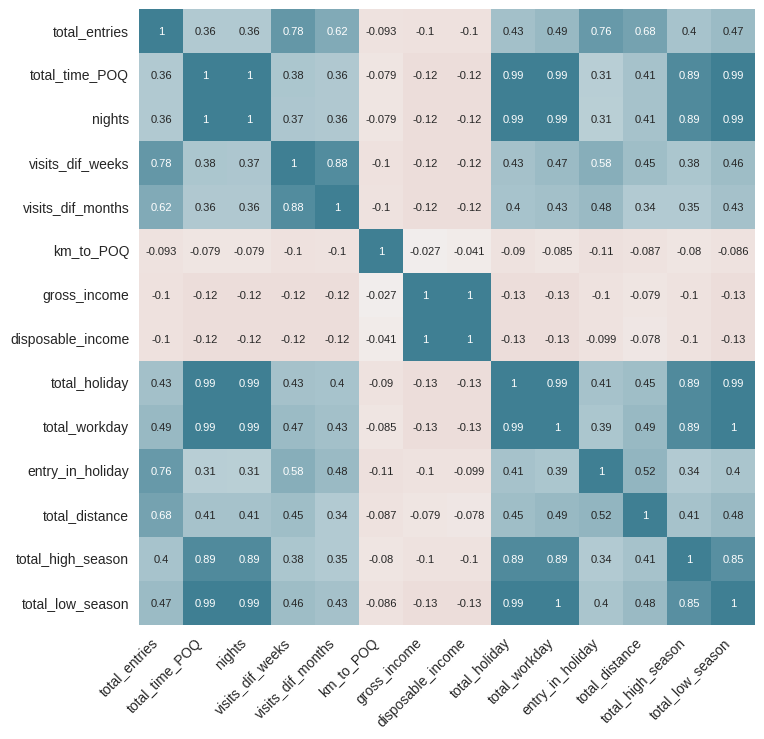
\includegraphics[width = \linewidth]{Images/matriz_corr_v2.png}
\end{center}
	\caption{\label{fig:matrix} Correlation matrix for all variables in the proposed dataset.}
\end{figure}

After applying the four most common normalization to the data (see in Chapter \ref{ch:fundamentals}), we apply PCA analysis. \cref{fig:pca-norms} shows the variance carried by each PCA component for each normalization. We can appreciate that two components explain most of the variance in all normalization. Hence, we perform an exploratory visual analysis plotting the first two principal components to study their underlying geometry. We have overlapped on the plots, in red, the points representing the vehicles of the registered residents. These visualizations provide information about the data structures and the performance of each normalization method. Based on the principal component analysis and the visualization of the data geometry, we will choose which type of algorithm and normalization is the most suitable for our problem (see in \cref{fig:plot-norms}).

\begin{figure}
    \centering
    \subfigure[Min-max normalization.]{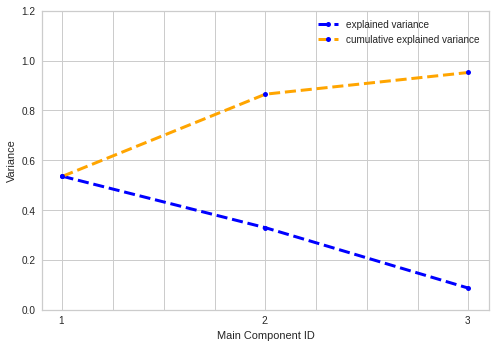
\includegraphics[width=0.49\textwidth]{Images/pca-max.png}}
    \subfigure[Z-score standarization.]{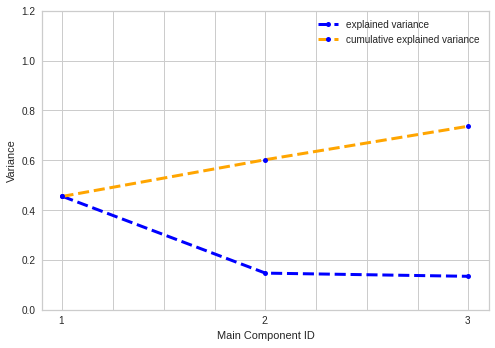
\includegraphics[width=0.49\textwidth]{Images/pca-mean.png}} 
    \subfigure[MAD normalization.]{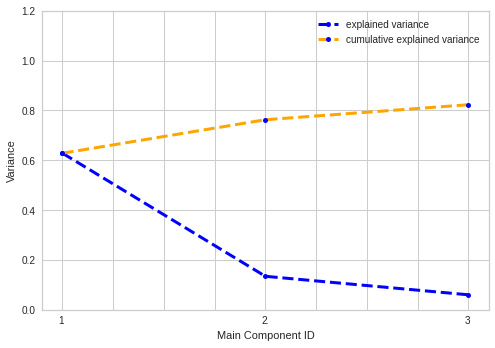
\includegraphics[width=0.49\textwidth]{Images/pca-mad.png}} 
    \subfigure[$\ell^2$ normalization.]{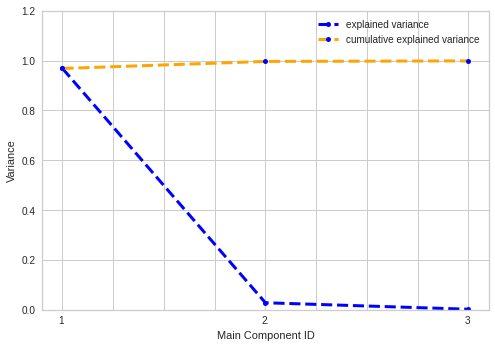
\includegraphics[width=0.49\textwidth]{Images/pca-l2.png}}
    \caption{Variance with 3 principal components.}
    \label{fig:pca-norms}
\end{figure}

\begin{figure}
    \centering
    \subfigure[Min-max normalization.]{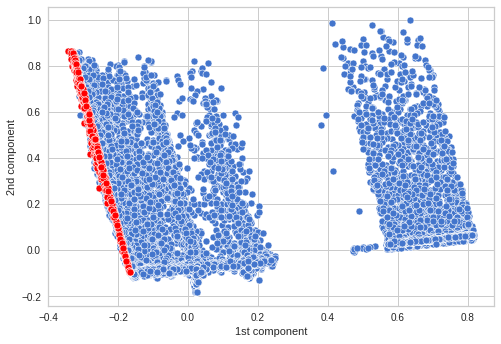
\includegraphics[width=0.49\textwidth]{Images/plot-max.png}}
    \subfigure[Z-score standarization.]{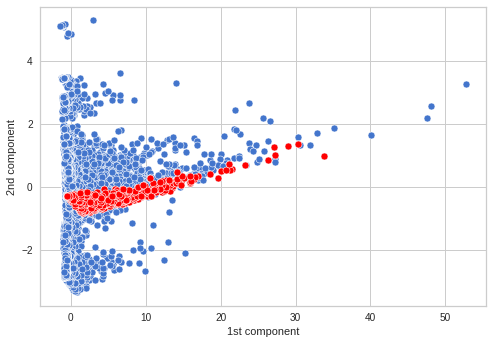
\includegraphics[width=0.49\textwidth]{Images/plot-mean.png}} 
    \subfigure[MAD normalization.]{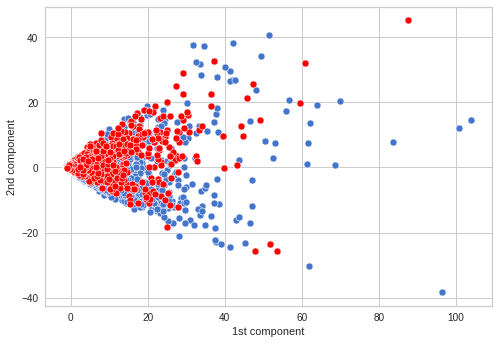
\includegraphics[width=0.49\textwidth]{Images/plot-mad.png}} 
    \subfigure[$\ell^2$ normalization.]{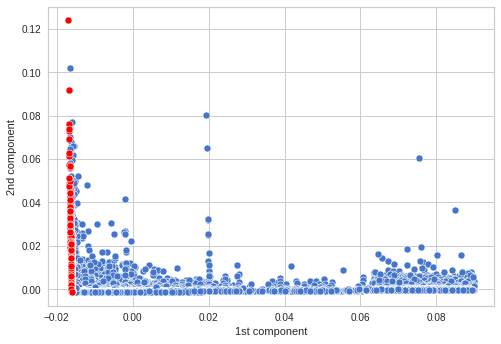
\includegraphics[width=0.49\textwidth]{Images/plot-l2.png}}
    \caption{Scatter-plot of the first two principal components for the different normalizations.}
    \label{fig:plot-norms}
\end{figure}

The normalization method that obtained the highest cumulative variance is $\ell^2$, indicating that it retains the most information in only two components (see in \cref{fig:pca-norms} (d)). In addition, the variance of each dimension is high compared to the other techniques analyzed, suggesting that the data are well distributed in both dimensions. The graph in \cref{fig:plot-norms} (d) shows a clear separation between the two groups, and the registered residents (in red) are well confined. The min-max normalization method obtained the second-best cumulative variance and the highest variance for each dimension, preserving a reasonable amount of information in only two components (see in \cref{fig:pca-norms} (a)). The graph also shows a clear separation between the two groups, and the actual residents are defined along a vertical line on the left cluster in \cref{fig:plot-norms} (a). In contrast, the mad normalization method has a lower cumulative variance and variance for each dimension (see in \cref{fig:pca-norms} (c)) than the $\ell^2$ and min-max normalization methods. The 2-dimensional scatter plot shows no apparent clusters (see in \cref{fig:plot-norms} (c)), and the actual residents are highly dispersed, which makes it unusable for our analysis. We had similar results in a scatter plot of three principal components. Finally, the mean normalization, z-score, method presented the lowest cumulative variance, indicating that it loses more information during dimensionality reduction than other techniques (see in \cref{fig:pca-norms} (b)). The graph shows that the actual residents are grouped together, but for the 2-components, there are no apparent significant clusters (see in \cref{fig:plot-norms} (c)). The trend of the cumulative variance explained is rising, suggesting that the current normalization method could be enhanced by including more components. By adding more dimensions, it may be possible to identify a dimension where the group of registered residents conforms to a clearer distribution. Principal Component Analysis (PCA) typically works better with z-score standardization than with min-max normalization. However, normalization techniques that better handle outliers (such as z-score) may not always be effective for all datasets because it tries to distribute the individuals uniformly, softening the outliers. For example, we observed that the min-max normalization method performed better than the z-score standardization, possibly due to the presence of small clusters that z-score detects as outliers. In particular, the dataset has a low proportion of registered residents (less than 2\% of the total sample), which could be considered outliers (see in \cref{tab:outliers}). In these cases, the min-max normalization method, which is more sensitive to small clusters, may give better results. With all this information, we decided to apply the two best normalizations for our data ($\ell^2$ and min-max) and compare the results obtained in the clustering.

From the scatter plots in \cref{fig:plot-norms}, we observe that the data points are spread relatively flat. This suggests that the data points are concentrated in a lower dimensional space within the original feature space. In other words, the data appears to exist in a more compressed space rather than being spread out across multiple dimensions. Hence, partition and distribution-based clustering models are the most suitable for this geometry (see in Section \ref{sec:flat}). To verify this, we have also tested other algorithms with poor results. For example, density and spectral-based algorithms performed poorly, probably because of the non-flat geometry, but also because they work best for detecting outliers. Hierarchical algorithms performed poorly, probably because of the non-flat geometry, but also they have difficulties with highly concentrated datasets, creating distinct groups only when the separation is very obvious. Consequently, we decided to focus on the partitional and distribution-based algorithms, which work well with flat geometry data. In particular, we try Gaussian mixtures, K-Means, and MiniBatchKMeans.

Gaussian Mixture models are more flexible and can handle different cluster shapes and sizes, while K-Means assumes a spherical shape of the clusters and a uniform size. In addition, Gaussian Mixture models can estimate the probability that a data point belongs to a cluster, which can be useful in specific applications where we need to make decisions based on uncertain data or when we want to assign a data point to multiple clusters with different probabilities. On the tests carried out, we discovered that K-Means and MiniBatchKMeans are not able to find any cluster that contains the majority of individuals of registered residents (see in \cref{fig:plot-norms} (a) and (d)). This is because the distribution of these individuals follows an elliptical geometry, which is not amenable to partition-based algorithms directly. Based on these results, we used the Gaussian Mixture clustering algorithm given the geometry of our data and the distribution followed by registered residents. 

\subsubsection*{Evaluation results}

Once selected the algorithm, we need to select the configuration and hyperparameters of the algorithm. In GaussianMixture algorithm, a ``mixture" refers to a linear combination of several Gaussian distributions, where each component represents a Gaussian distribution in the mixture \cite{Reynolds2009}. Each mixture component is defined by a set of parameters, including its own mean and covariance matrix, which describes how the data are distributed in that space. In practice, the number of mixture components is an adjustable parameter of the algorithm, meaning that we can specify how many Gaussian distributions to combine to model the data. Another configurable parameter of the GaussianMixture algorithm covariance type used to construct the covariance matrix associated with each mixture component. These covariance types specify how the different variables in the data are correlated and can significantly affect the accuracy and efficiency of the model. The common types of covariance are:

\begin{itemize}
    \item Full: all components have their own covariance matrix. This means that each component can have a complex correlation structure between the different variables.
    \item Tied: all components share the same overall covariance matrix. This can be useful if different variables are highly correlated.
    \item Diagonal: each component has its own diagonal in the covariance matrix. This means that the correlation structure between the different variables is limited to correlations between pairs of variables.
    \item Spherical: each mixture component has its own unique variance. This means that the correlation structure between the different variables is limited to the variance of each variable individually.
\end{itemize}

To select the best hyperparameters, we calculate the performance of the resulting model with the metrics presented in Section \ref{subsec:algorithms-mets}, which are appropriated for clustering algorithms based on density (BIC and AIC). In the next subsections, we perform the evaluation for the different types of covariance of the GaussianMixture algorithm on the two normalizations chosen in the previous subsection: min-max and $\ell^2$ normalization.


\subsubsection*{Evaluation results: Min-max normalization}

We begin first by presenting the results obtained with the min-max normalization. \cref{fig:plot-mixmax-bic} represents the values of the BIC and AIC metrics with respect to the number of components and type of covariance used as parameters of the GaussianMixture algorithm. We note that the ``full" covariance type is the one that minimizes both metrics in all cases, so it will be the one chosen for the subsequent analysis. This value means that each component has its own overall covariance matrix, which means it can capture any correlation between variables. We note no significant differences between the values obtained for AIC and BIC scores. Therefore, we calculate the elbow method on the BIC score to select the optimal number of mixture components, which from \cref{fig:plot-mixmax-elbow} is 7, producing an abrupt change in the slope of the curve.

\begin{figure}
    \centering
    \subfigure[BIC score.]{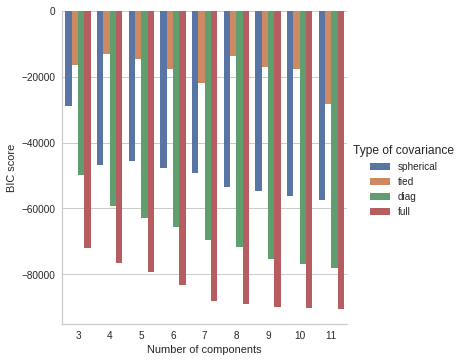
\includegraphics[width=0.49\textwidth]{Images/bic_minmax_2.png}}
    \subfigure[AIC score.]{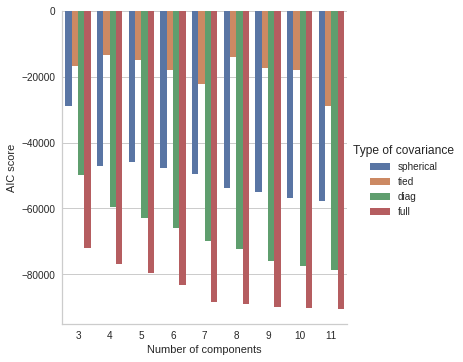
\includegraphics[width=0.49\textwidth]{Images/aic_minmax_2.png}} 
    \caption{Information criteria for the GaussianMixture on min-max normalization.}
    \label{fig:plot-mixmax-bic}
\end{figure}

\begin{figure}
    \centering
    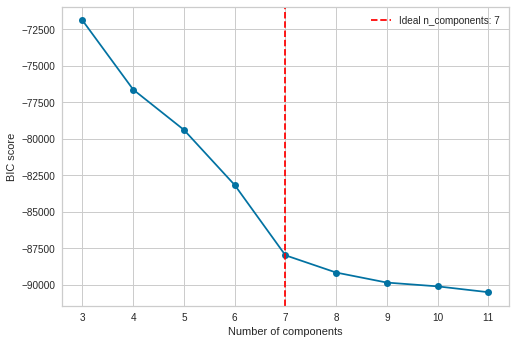
\includegraphics[width=0.6\textwidth]{Images/bic_minmax_elbow_2.png}
    \caption{Elbow method for BIC using min-max normalization.}
    \label{fig:plot-mixmax-elbow}
\end{figure}

\subsubsection*{Evaluation results: $\ell^2$ normalization}

\cref{fig:plot-l2-bic} represents the values of the BIC and AIC metrics with respect to the number of components and type of covariance, used as parameters of the GaussianMixture algorithm for $\ell^2$ normalization. We observe that the ``tied'' covariance type is slightly superior for 3 components, although for more than 3 components the ``full'' covariance type is again the best. Similarly to the min-max normalization, there is no significant difference between the values obtained for AIC and BIC scores. Therefore, we will calculate the elbow method on the BIC score (see in \cref{fig:plot-l2-bic}) and ``full'' covariance type. The elbow method indicates that there is a sharp change in the slope at 4 components.


\begin{figure}
    \centering
    \subfigure[BIC score.]{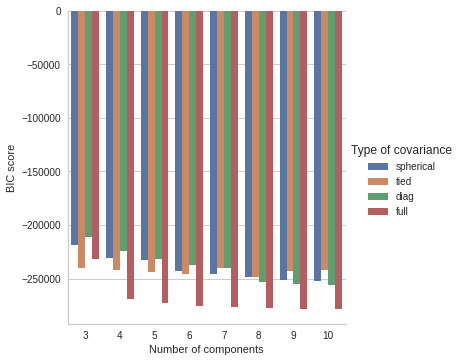
\includegraphics[width=0.49\textwidth]{Images/bic_l2.png}}
    \subfigure[AIC score.]{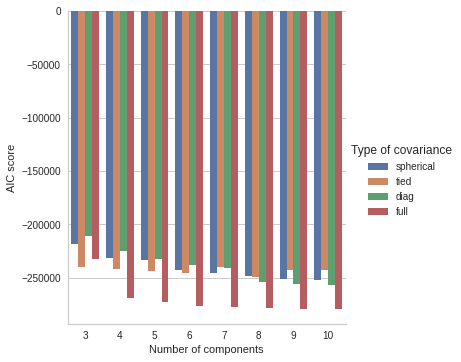
\includegraphics[width=0.49\textwidth]{Images/aic_l2.png}} 
    \caption{Information criteria for the GaussianMixture on $\ell^2$ normalization.}
    \label{fig:plot-l2-bic}
\end{figure}

 

\begin{figure}
    \centering
    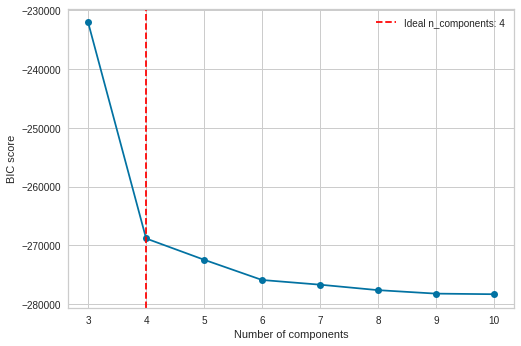
\includegraphics[width=0.6\textwidth]{Images/bic_l2_elbow.png}
    \caption{Elbow method for BIC using $\ell^2$ normalization.}
    \label{fig:plot-l2-elbow}
\end{figure}

\subsubsection*{Visualization results}

Once we have selected the clustering algorithm and the hyperparameters, we will discuss the visualization of the generated clusters over the two chosen normalizations: min-max normalization and $\ell^2$.  

\subsubsection*{Visualization: Min-max normalization}

\cref{fig:plot-scatter-min-max} (a) shows a 2D scatter plot, where each axis represents one of the principal components (1st and 2nd) of the distribution. In \cref{fig:plot-scatter-min-max} (b), we highlight in red the registered residents labeled in our database. Finally, in \cref{fig:plot-scatter-min-max} (c), we can visualize the 3D scatter plot, in which each axis represents one of the 3 principal components. \cref{tab:minmax-perc}, shows the percentage of vehicles and the number of registered residents in each of the 7 clusters. We can see that cluster 3 correctly groups more than 96\% of this group of individuals. Approximately 48\% of the total sample is grouped in only one cluster (cluster 5), so almost half of the vehicles follow the same behavior. In addition, the cluster containing most of the registered residents (cluster 3) represents approximately 11\% of the total population.

\begin{figure}
    \centering
    \subfigure[Segmentation for 7 mixture components.]{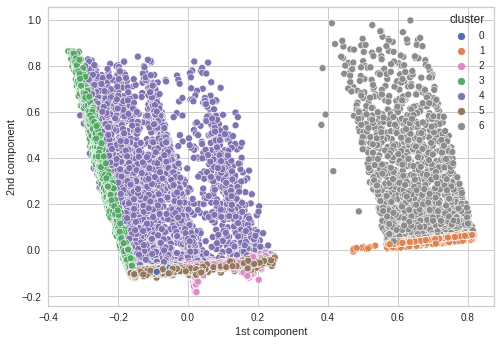
\includegraphics[width=0.49\textwidth]{Images/clustering_sinred_minmax.png}}
    \subfigure[Highlighted registered residents.]{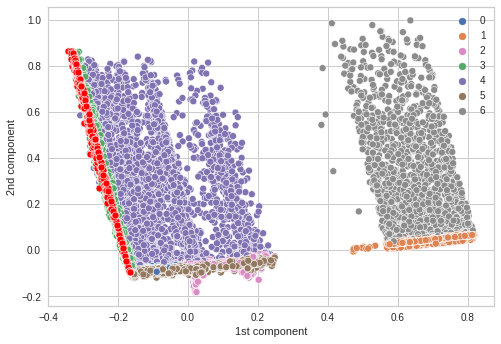
\includegraphics[width=0.49\textwidth]{Images/clustering_red_minmax.png}} 
    \subfigure[3D plot with 3rd component.]{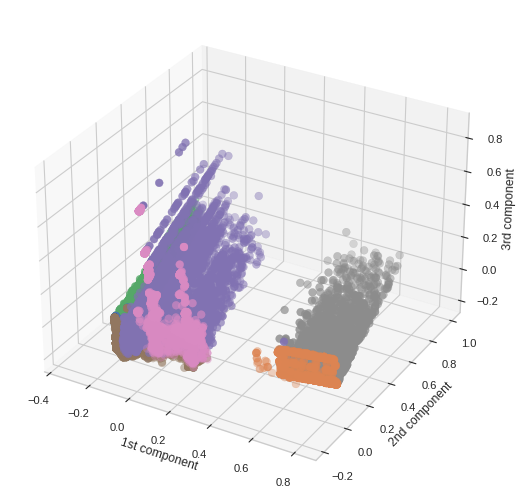
\includegraphics[width=0.49\textwidth]{Images/visual_3D_minmax.png}} 
    \caption{Scatter-plot of the first three components (PCA) using min-max normalization.}
    \label{fig:plot-scatter-min-max}
\end{figure}

% Please add the following required packages to your document preamble:
% \usepackage{graphicx}
\begin{table}[]
\centering
\resizebox{\columnwidth}{!}{%
\begin{tabular}{cccccccc}
\hline
Data points          & \multicolumn{7}{c}{Nº cluster}                                  \\ \hline
                     & 0       & 1      & 2      & 3       & 4      & 5       & 6      \\ \hline
Percentage of sample & 15.04\% & 6.11\% & 8.58\% & 11.17\% & 8.55\% & 47.50\% & 3.05\% \\ \hline
Real Residents       & 10      & 0      & 0      & 641     & 3      & 12      & 0      \\ \hline
Rest of individuals  & 7391    & 3009   & 4221   & 4862    & 4205   & 23,370  & 1500   \\ \hline
\end{tabular}%
}
\caption{Clusters based on registered resident labels using min-max normalization.}
\label{tab:minmax-perc}
\end{table}

\cref{fig:boxplot-minmax} presents the box plots for the 7 clusters for the nights (\cref{fig:boxplot-minmax} (a)) and km\_to\_POQ (\cref{fig:boxplot-minmax} (b)) variables, which show significant differences in explaining the groups. \cref{fig:boxplot-minmax-1,fig:boxplot-minmax-2} present the box plots of the most relevant variables for the 7 clusters obtained, making a previous division into 2 groups, which we explain below. \cref{tab:means-minmax} complements \cref{fig:boxplot-minmax-1,fig:boxplot-minmax-2}, indicating the exact number of the mean of each variable in each cluster. To facilitate visualization, we have separated some of the box plots according to the value of the variable nights, which seems to discriminate well between 2 groups of clusters: (0, 1, 2, 5) with lower values and (3, 4, 6) with higher values (see in \cref{fig:boxplot-minmax} (a)). Clusters 3,4,6 have a number of nights close to the behavior of a resident in the area. These represent 22.77\% of the total sample (see in \cref{tab:minmax-perc}). Clusters 0,1,2,5 have visitor behavior because they spent fewer nights in the area and represent 77.23\% of the total dataset. Thus, we can define a distinction between the 7 clusters based on length of stay, which is directly correlated with overnights.

\begin{figure}
    \centering
    \subfigure[Total nights of stay by cluster.]{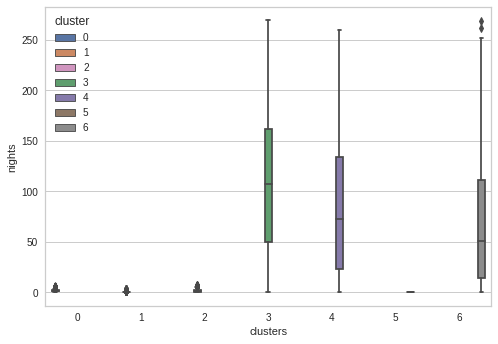
\includegraphics[width=0.49\textwidth]{Images/boxplot_minmax_1.png}}
    \subfigure[Distance in Km. to the area by cluster.]{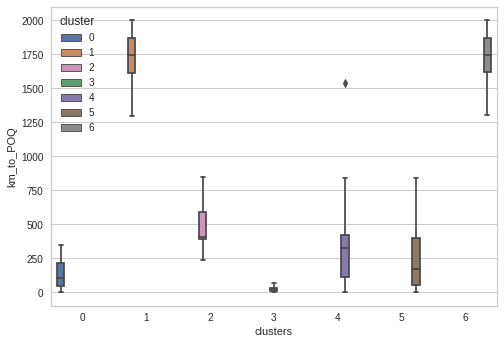
\includegraphics[width=0.49\textwidth]{Images/boxplot_minmax_2.png}}
    \caption{box plots for min-max normalization (I).}
    \label{fig:boxplot-minmax}
\end{figure}


\begin{figure}
    \centering
    \subfigure[Nights of stay for clusters \textbf{3,4,6}.]{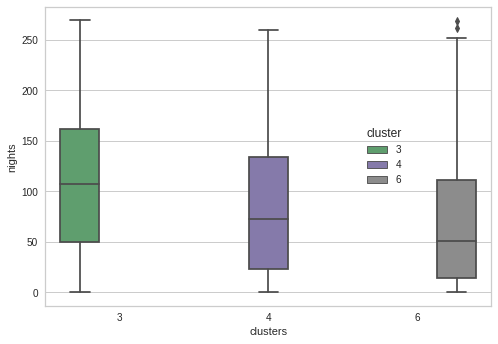
\includegraphics[width=0.49\textwidth]{Images/boxplot_max_1.png}}
    \subfigure[Nights of stay for clusters \textbf{0,1,2,5}.]{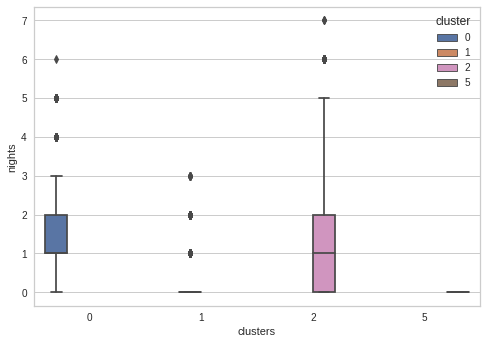
\includegraphics[width=0.49\textwidth]{Images/boxplot_min_1.png}}
    \subfigure[Distance to the area for clusters \textbf{3,4,6}.]{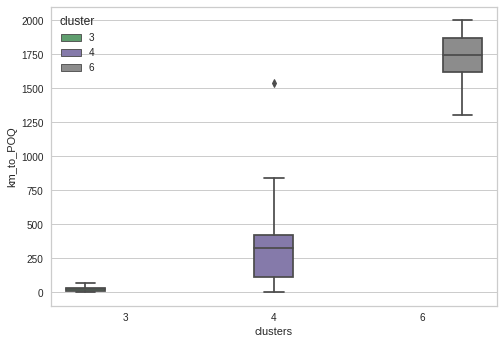
\includegraphics[width=0.49\textwidth]{Images/boxplot_max_2.png}}
    \subfigure[Distance to the area for clusters \textbf{0,1,2,5}.]{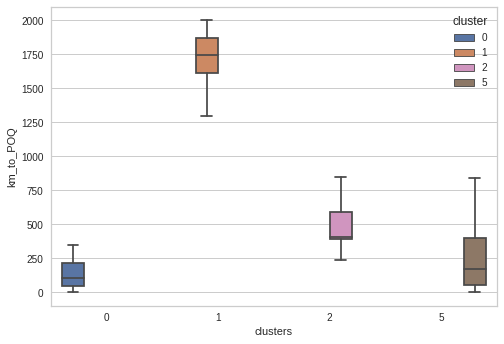
\includegraphics[width=0.49\textwidth]{Images/boxplot_min_2.png}}
    \subfigure[Total entries for clusters \textbf{3,4,6}.]{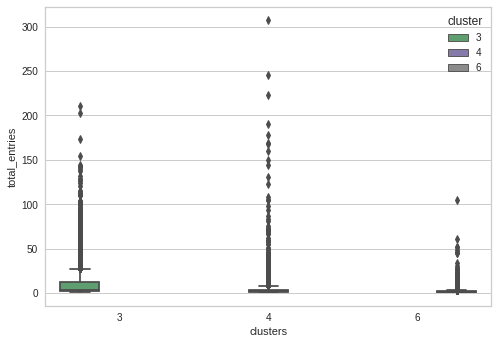
\includegraphics[width=0.49\textwidth]{Images/boxplot_max_3.png}} 
    \subfigure[Total entries for clusters \textbf{0,1,2,5}.]{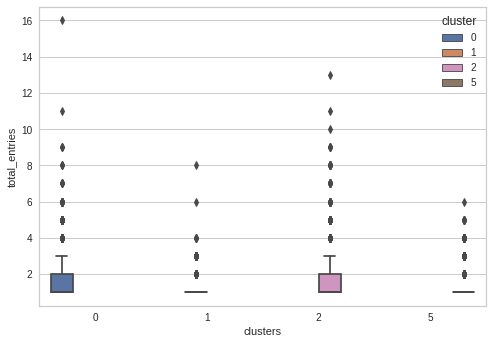
\includegraphics[width=0.49\textwidth]{Images/boxplot_min_3.png}} 
    \caption{Box plots for min-max normalization (II).}
    \label{fig:boxplot-minmax-1}
\end{figure}

\begin{figure}
    \centering
    \subfigure[Distance run in area for clusters \textbf{3,4,6}.]{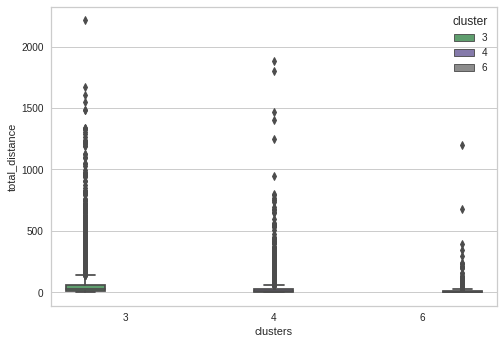
\includegraphics[width=0.49\textwidth]{Images/boxplot_max_4.png}}
    \subfigure[Distance run in area for clusters \textbf{0,1,2,5}.]{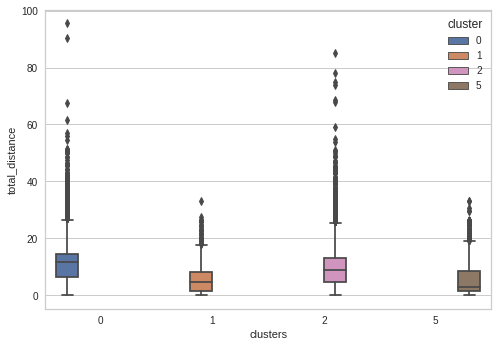
\includegraphics[width=0.49\textwidth]{Images/boxplot_min_4.png}}
    \subfigure[Avg. gross income for clusters \textbf{3,4,6}.]{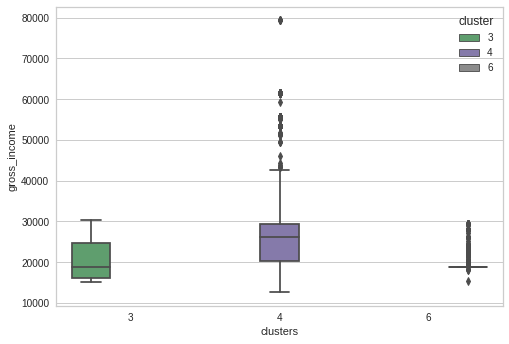
\includegraphics[width=0.49\textwidth]{Images/boxplot_max_5.png}} 
    \subfigure[Avg. gross income for clusters \textbf{0,1,2,5}.]{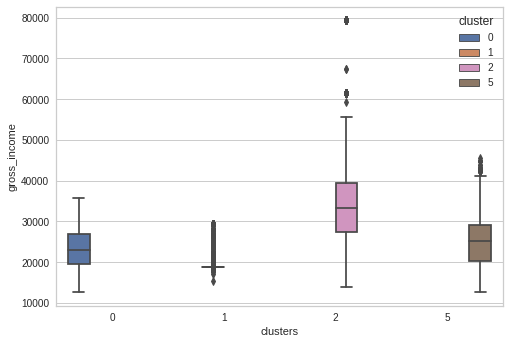
\includegraphics[width=0.49\textwidth]{Images/boxplot_min_5.png}} 
    \subfigure[Total high season for clusters \textbf{3,4,6}.]{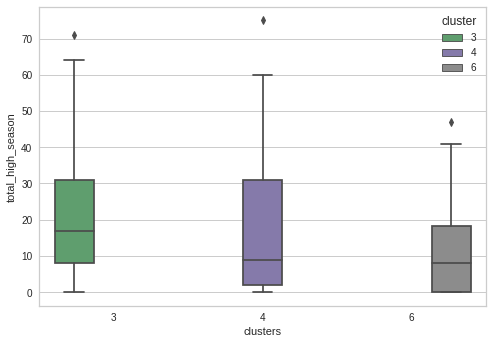
\includegraphics[width=0.49\textwidth]{Images/boxplot_max_6.png}} 
    \subfigure[Total high season for clusters \textbf{0,1,2,5}.]{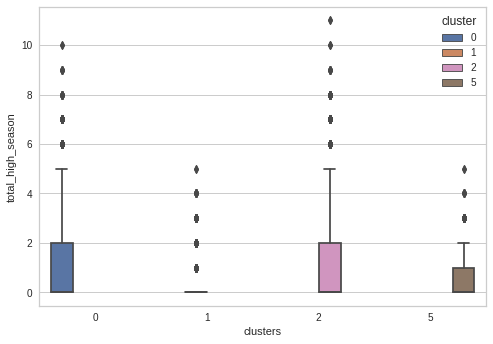
\includegraphics[width=0.49\textwidth]{Images/boxplot_min_6.png}} 
    \caption{Box plots for min-max normalization (III).}
    \label{fig:boxplot-minmax-2}
\end{figure}

For clusters 3,4,6 (residents' behavior), another relevant variable is the distance in kilometers from the registered address of the vehicle to the area (see in \cref{fig:boxplot-minmax-1} (c)). The three clusters, despite having notable differences for the variable of origin, have similar behaviors for the variable of nights. Hence, the individuals in these 3 clusters have residence or accommodation in the area. According to their distance to the area, cluster 3, with a mean value of 19.39 km (see in \cref{tab:means-minmax}), corresponds mostly to vehicles registered in the area under study (registered residents) and nearby villages in the Alpujarra. Cluster 6, with a mean value of 1747.30 km for the variable km\_to\_POQ, corresponds to non-registered residents from abroad that we defined in Section \ref{sec:smartvillages}. Cluster 4, with a mean value of 318.36 km, corresponds to individuals from other regions of Spain who are non-registered residents, which we also discussed in that Section. Moreover, the gross income variable is much higher in group 4 than in groups 3 and 6 (almost 34\% higher) (see in \cref{fig:boxplot-minmax-2} (c)). Therefore, we can say that the majority of individuals in this group (non-registered residents from other Spanish regions) come from regions with higher incomes than the average of the rest of the residents. We can observe that in general for the three groups of residents, the mean of the variables total\_distance, total\_high\_season, and total\_entries (see in \cref{tab:means-minmax}), are inversely proportional to the mean of the clusters for the variable km\_to\_POQ. Therefore, residents coming from farther away (clusters 4 and 6) will have a lower mean than the clusters coming from closer (cluster 3) for those variables, this is because coming from farther away the frequency of visitation, kilometers traveled and visits in high season (see in \cref{fig:boxplot-minmax-1} (e) and \cref{fig:boxplot-minmax-2} (a, e)) will also be lower.

For clusters 0,1,2,5 (visitor behavior), we also describe the average behavior of each cluster (see in \cref{tab:means-minmax}). Cluster 0 has an average distance of 128.55 km to the area, so it corresponds to visitors from the province of Granada (region of the villages). This cluster comprises individuals who spend an average of 1.57 nights in the area. The variable total\_entries tells us that individuals have made an average of 1.54 visits during the period collected in the sample. Due to its variables total\_high\_season (see in \cref{fig:boxplot-minmax-2} (b, f)), we observe that more than 65\% of the visits are made in high season. Therefore, this cluster corresponds to individuals from the province of Granada who visit the area on weekends and holidays and stay between 1–2 nights. Cluster 1 has an average of 1742.97 km, which indicates foreign visitors. This cluster has an average of 0.26 nights, so they are individuals who usually visit the area during the day. Observing the variable total\_high\_season, we can see that the behavior of these individuals who come from abroad is to visit in low seasons. In addition, the relatively low value of the total\_distance variable (4.90 km) suggests that it is likely that these tourists visit one of the three villages, specifically Pampaneira, using the main road instead of deviating from other routes, probably the behavior of these individuals is to visit the towns of the Alpujarra that coincide with the route of the main road. Cluster 2 has an average of 474.21 km, so visitors come from outside the province of Granada. This cluster comprises individuals who spend an average of 1.55 nights in the area, similar to cluster 0 (visitors from the province of Granada). This cluster has the highest average for the gross\_income variable of all the clusters (see in \cref{fig:boxplot-minmax-2} (d)). This leads us to think that it contains vehicles from the north of Spain, where the average income is higher than in the south of Spain. In addition, the variable total\_high\_season, shows that approximately 74\% of the stays are in high season, so these individuals correspond to tourists from the northern regions of Spain who decide to spend 1–2 days in the Alpujarra during their holidays. Finally, cluster 5 has an average of 253.70 km, indicating visitors from other Andalusia provinces. This cluster has an average of 0 nights, so the visits usually occur during the day, with no associated overnight stays. It is important to highlight that cluster 5 represents 47.50\% of the individuals in the sample (see in \cref{tab:minmax-perc}), so we can say that the majority behavior among individuals is not to spend the night in the area. Furthermore, they rarely come in high season (27\% of the total entries) (see in \cref{fig:boxplot-minmax-2} (f)), so the majority will correspond to tourists from other provinces of Andalusia who visit the area and return home at the end of the day.

\begin{table}[]
\centering
\resizebox{\columnwidth}{!}{%
\begin{tabular}{cccccccc}
\hline
Variables           & \multicolumn{7}{c}{Nº cluster}                                                    \\ \hline
                    & 0         & 1         & 2         & 3         & 4         & 5         & 6         \\ \hline
nights              & 1.57      & 0.26      & 1.55      & 108.62    & 84.66     & 0.00      & 68.73     \\ \hline
km\_to\_POQ         & 128.55    & 1742.97   & 474.21    & 19.39     & 318.36    & 253.70    & 1747.30   \\ \hline
total\_entries      & 1.54      & 1.12      & 1.58      & 10.34     & 4.36      & 1.12      & 2.71      \\ \hline
total\_distance     & 11.64     & 4.90      & 10.67     & 70.24     & 30.77     & 4.86      & 14.42     \\ \hline
gross\_income       & 23,085.36 & 19,482.10 & 35,547.66 & 20,972.17 & 26,902.26 & 25,151.75 & 19,179.54 \\ \hline
total\_high\_season & 1.01      & 0.31      & 1.14      & 18.85     & 15.10     & 0.31      & 11.24     \\ \hline
\end{tabular}%
}
\caption{Mean of variables for each cluster performed using min-max normalization.}
\label{tab:means-minmax}
\end{table}

\subsubsection*{Visualization: $\ell^2$ normalization}

\cref{fig:plot-scatter-l2} shows the distribution of the data using the $\ell^2$ normalization. \cref{fig:plot-scatter-l2} (a) shows a 2D scatter plot, where each axis represents one of the principal components (1st and 2nd) of the distribution of the groups. In \cref{fig:plot-scatter-l2} (b), we highlight in red the registered residents. Finally, in \cref{fig:plot-scatter-l2} (c), we can visualize the 3D scatter plot. \cref{tab:l2-perc} shows the percentage of the total sample and the number of registered residents in each cluster. We can see cluster 0 correctly groups more than 88\% of the registered residents. Approximately 80\% of the total sample is grouped in a single cluster (cluster 3). In addition, the cluster containing registered residents (cluster 0) represents approximately 9\% of the total population.

\begin{figure}
    \centering
    \subfigure[Segmentation for 4 mixture components.]{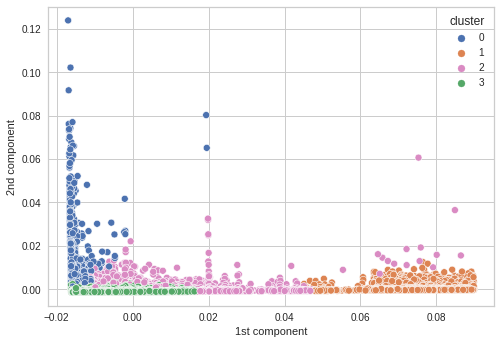
\includegraphics[width=0.49\textwidth]{Images/clustering_sinred_l2.png}}
    \subfigure[Highlighted registered residents.]{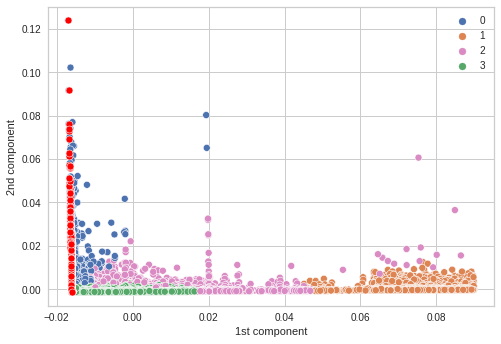
\includegraphics[width=0.49\textwidth]{Images/clustering_red_l2.png}} 
    \subfigure[3D plot with 3rd component.]{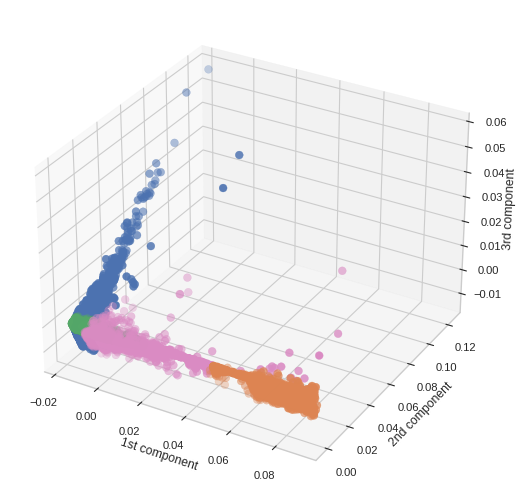
\includegraphics[width=0.49\textwidth]{Images/visual_3D_l2.png}} 
    \caption{Scatter-plot of the first three components (PCA) using $\ell^2$ normalization.}
    \label{fig:plot-scatter-l2}
\end{figure}


\begin{table}[]
%\centering
\resizebox{9cm}{!} & \multicolumn{1}{l}{8.76\%} & \multicolumn{1}{l}{4.36\%} & \multicolumn{1}{l}{78.33\%} \\ \hline
Real Residents                           & 589                        & 0                          & 0                          & 77                          \\ \hline
Rest of individuals                      & 3620                       & 4314                       & 2146                       & 38,478                      \\ \hline
\end{tabular}%
}
\caption{Clusters based on actual resident labels using $\ell^2$ normalization.}
\label{tab:l2-perc}
\end{table}

\cref{fig:boxplot-l2} shows the box plots of the relevant variables for the 4 clusters, and \cref{tab:means-l2} shows the mean of each of these variables in each cluster. We distinguish two clusters that contain a high value of the variable nights (cluster 0 and 2), while the rest of the clusters (clusters 1 and 3) have a low value. Although there are outliers (see in \cref{fig:boxplot-l2} (a)) that increase the mean number of nights for these clusters (clusters 1 and 3), 50\% of the individuals have a number of nights lower than 2 for cluster 3 and lower than 15 nights for cluster 1. 

Cluster 0 has an average of 144.93 nights and an average distance to the area of 25.54 km. In addition, it contains more than 88\% of the real residents. hence, we can consider this cluster as that of the area's residents (registered and unregistered). Most of the unregistered residents in this group, as shown in \cref{fig:boxplot-l2} (b), come from the province of Granada. Cluster 2 is small (only 4.36\% of the total sample) of non-registered residents who spend an average of 84.62 nights and come from an average origin of 598.01 km. Therefore, it corresponds to residents from outside the province of Granada. We can observe that in general, for the two groups, the means of the variables total\_distance, total\_high\_season and total\_entries (see in \cref{tab:means-l2}), are inversely proportional to the means of the variable km\_to\_POQ. This means that visitors that come from further away tend to: visit in the low season; move less inside the area; and come fewer times in the year than other visitors (see in \cref{fig:boxplot-l2} (c, d, f)). Cluster 1 comprises individuals from afar to the 1750.68 km area and has an average of 22.81 nights (although most of them spend less than two nights). This group contains foreign visitors and some unregistered foreign residents (less than half of the group). Only 17\% of the stays are in high season. This is because the cluster comprises foreigners, so they do not depend on the Spanish national calendar. Furthermore, despite having an average of 22.81 nights, the visits to the area are only 1.52, which means that in all those days they do not travel to nearby areas (see in \cref{tab:means-l2}). Finally, group 3 contains the majority of individuals in the data set and models individuals with a mean behavior of 4.82 nights (although most do not stay overnight) and 240.01 km of distance. This cluster represents 78.33\% of the individuals in the sample (see in \cref{tab:l2-perc}). Hence, we can say that the majority behavior of the individuals is not to spend the night in the area. In addition, they rarely come in high season (28\% of the total stay) (see in \cref{fig:boxplot-l2} (f)). Thus, the majority will correspond to tourists from Granada and other nearby Andalusian provinces visiting the area and returning home at the end of the day. Cluster 3 has the highest income, with a mean of 26,158.32; however, since it contains almost 80\% of the sample, it does not provide much information.

\begin{figure}
    \centering
    \subfigure[Total nights of stay by cluster.]{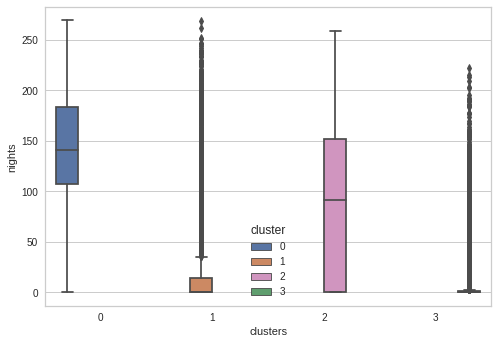
\includegraphics[width=0.49\textwidth]{Images/boxplot_l2_1.png}}
    \subfigure[Distance in Km. to the area by cluster.]{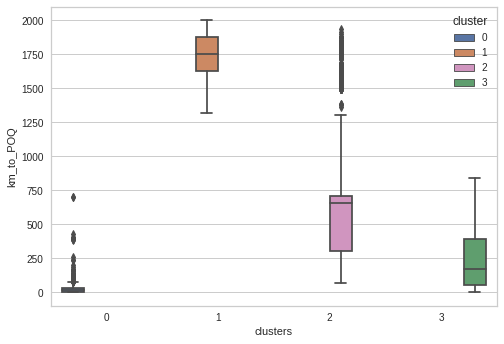
\includegraphics[width=0.49\textwidth]{Images/boxplot_l2_2.png}} 
    \subfigure[Total entries to the area by cluster.]{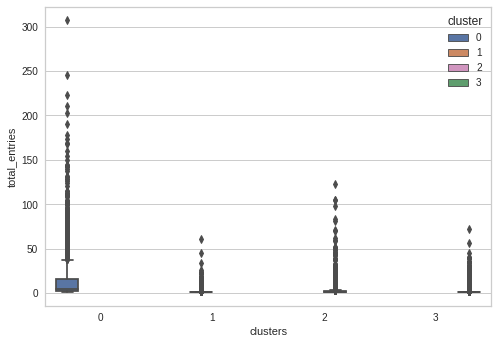
\includegraphics[width=0.49\textwidth]{Images/boxplot_l2_3.png}}
    \subfigure[Distance run in area by cluster.]{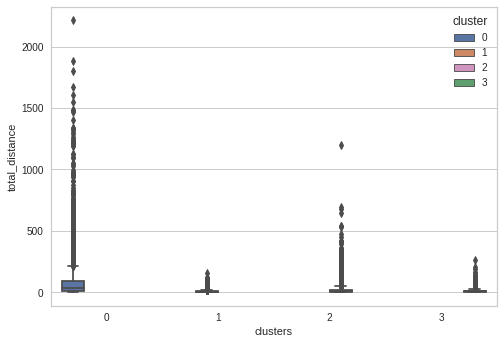
\includegraphics[width=0.49\textwidth]{Images/boxplot_l2_4.png}} 
    \subfigure[Average gross income by cluster.]{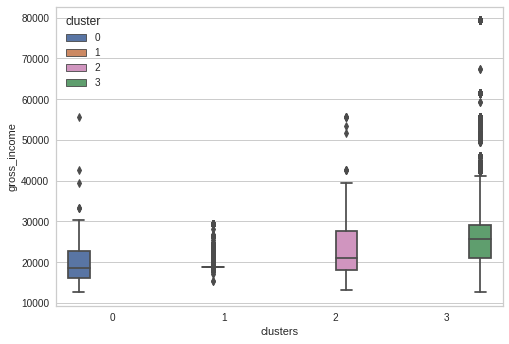
\includegraphics[width=0.49\textwidth]{Images/boxplot_l2_5.png}} 
    \subfigure[Total high season by cluster.]{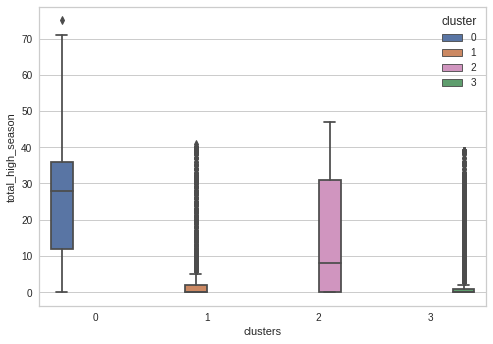
\includegraphics[width=0.49\textwidth]{Images/boxplot_l2_6.png}} 
    \caption{Box plots for $\ell^2$ normalization.}
    \label{fig:boxplot-l2}
\end{figure}

\begin{table}[]
%\centering
\resizebox{10cm}{!}{%
\begin{tabular}{ccccc}
\hline
Variables           & \multicolumn{4}{c}{Nº cluster}                \\ \hline
                    & 0         & 1         & 2         & 3         \\ \hline
nights              & 144.93    & 22.81     & 84.62     & 4.82      \\ \hline
km\_to\_POQ         & 25.54     & 1750.68   & 598.01    & 240.01    \\ \hline
total\_entries      & 13.18     & 1.52      & 3.53      & 1.49      \\ \hline
total\_distance     & 95.43     & 6.89      & 26.43     & 8.01      \\ \hline
gross\_income       & 20,268.41 & 19,018.55 & 22,886.88 & 26,158.32 \\ \hline
total\_high\_season & 24.83     & 3.87      & 14.47     & 1.36      \\ \hline
\end{tabular}%
}
\caption{Mean of variables for each cluster performed using $\ell^2$ normalization.}
\label{tab:means-l2}
\end{table}